\documentclass[a4paper,12pt,twoside]{memoir}

% Castellano
\usepackage[spanish,es-tabla]{babel}
\selectlanguage{spanish}
\usepackage[utf8]{inputenc}
\usepackage[T1]{fontenc}
\usepackage{lmodern} % Scalable font
\usepackage{microtype}
\usepackage{placeins}

\RequirePackage{booktabs}
\RequirePackage[table]{xcolor}
\RequirePackage{xtab}
\RequirePackage{multirow}

% Links
\PassOptionsToPackage{hyphens}{url}\usepackage[colorlinks]{hyperref}
\hypersetup{
	allcolors = {red}
}

% Ecuaciones
\usepackage{amsmath}

% Rutas de fichero / paquete
\newcommand{\ruta}[1]{{\sffamily #1}}

% Párrafos
\nonzeroparskip

% Huérfanas y viudas
\widowpenalty100000
\clubpenalty100000

% Imágenes

% Comando para insertar una imagen en un lugar concreto.
% Los parámetros son:
% 1 --> Ruta absoluta/relativa de la figura
% 2 --> Texto a pie de figura
% 3 --> Tamaño en tanto por uno relativo al ancho de página
\usepackage{graphicx}
\newcommand{\imagen}[3]{
	\begin{figure}[!h]
		\centering
		\includegraphics[width=#3\textwidth]{#1}
		\caption{#2}\label{fig:#1}
	\end{figure}
	\FloatBarrier
}

% Comando para insertar una imagen sin posición.
% Los parámetros son:
% 1 --> Ruta absoluta/relativa de la figura
% 2 --> Texto a pie de figura
% 3 --> Tamaño en tanto por uno relativo al ancho de página
\newcommand{\imagenflotante}[3]{
	\begin{figure}
		\centering
		\includegraphics[width=#3\textwidth]{#1}
		\caption{#2}\label{fig:#1}
	\end{figure}
}

% El comando \figura nos permite insertar figuras comodamente, y utilizando
% siempre el mismo formato. Los parametros son:
% 1 --> Porcentaje del ancho de página que ocupará la figura (de 0 a 1)
% 2 --> Fichero de la imagen
% 3 --> Texto a pie de imagen
% 4 --> Etiqueta (label) para referencias
% 5 --> Opciones que queramos pasarle al \includegraphics
% 6 --> Opciones de posicionamiento a pasarle a \begin{figure}
\newcommand{\figuraConPosicion}[6]{%
  \setlength{\anchoFloat}{#1\textwidth}%
  \addtolength{\anchoFloat}{-4\fboxsep}%
  \setlength{\anchoFigura}{\anchoFloat}%
  \begin{figure}[#6]
    \begin{center}%
      \Ovalbox{%
        \begin{minipage}{\anchoFloat}%
          \begin{center}%
            \includegraphics[width=\anchoFigura,#5]{#2}%
            \caption{#3}%
            \label{#4}%
          \end{center}%
        \end{minipage}
      }%
    \end{center}%
  \end{figure}%
}

%
% Comando para incluir imágenes en formato apaisado (sin marco).
\newcommand{\figuraApaisadaSinMarco}[5]{%
  \begin{figure}%
    \begin{center}%
    \includegraphics[angle=90,height=#1\textheight,#5]{#2}%
    \caption{#3}%
    \label{#4}%
    \end{center}%
  \end{figure}%
}
% Para las tablas
\newcommand{\otoprule}{\midrule [\heavyrulewidth]}
%
% Nuevo comando para tablas pequeñas (menos de una página).
\newcommand{\tablaSmall}[5]{%
 \begin{table}
  \begin{center}
   \rowcolors {2}{gray!35}{}
   \begin{tabular}{#2}
    \toprule
    #4
    \otoprule
    #5
    \bottomrule
   \end{tabular}
   \caption{#1}
   \label{tabla:#3}
  \end{center}
 \end{table}
}

%
% Nuevo comando para tablas pequeñas (menos de una página).
\newcommand{\tablaSmallSinColores}[5]{%
 \begin{table}[H]
  \begin{center}
   \begin{tabular}{#2}
    \toprule
    #4
    \otoprule
    #5
    \bottomrule
   \end{tabular}
   \caption{#1}
   \label{tabla:#3}
  \end{center}
 \end{table}
}

\newcommand{\tablaApaisadaSmall}[5]{%
\begin{landscape}
  \begin{table}
   \begin{center}
    \rowcolors {2}{gray!35}{}
    \begin{tabular}{#2}
     \toprule
     #4
     \otoprule
     #5
     \bottomrule
    \end{tabular}
    \caption{#1}
    \label{tabla:#3}
   \end{center}
  \end{table}
\end{landscape}
}

%
% Nuevo comando para tablas grandes con cabecera y filas alternas coloreadas en gris.
\newcommand{\tabla}[6]{%
  \begin{center}
    \tablefirsthead{
      \toprule
      #5
      \otoprule
    }
    \tablehead{
      \multicolumn{#3}{l}{\small\sl continúa desde la página anterior}\\
      \toprule
      #5
      \otoprule
    }
    \tabletail{
      \hline
      \multicolumn{#3}{r}{\small\sl continúa en la página siguiente}\\
    }
    \tablelasttail{
      \hline
    }
    \bottomcaption{#1}
    \rowcolors {2}{gray!35}{}
    \begin{xtabular}{#2}
      #6
      \bottomrule
    \end{xtabular}
    \label{tabla:#4}
  \end{center}
}

%
% Nuevo comando para tablas grandes con cabecera.
\newcommand{\tablaSinColores}[6]{%
  \begin{center}
    \tablefirsthead{
      \toprule
      #5
      \otoprule
    }
    \tablehead{
      \multicolumn{#3}{l}{\small\sl continúa desde la página anterior}\\
      \toprule
      #5
      \otoprule
    }
    \tabletail{
      \hline
      \multicolumn{#3}{r}{\small\sl continúa en la página siguiente}\\
    }
    \tablelasttail{
      \hline
    }
    \bottomcaption{#1}
    \begin{xtabular}{#2}
      #6
      \bottomrule
    \end{xtabular}
    \label{tabla:#4}
  \end{center}
}

%
% Nuevo comando para tablas grandes sin cabecera.
\newcommand{\tablaSinCabecera}[5]{%
  \begin{center}
    \tablefirsthead{
      \toprule
    }
    \tablehead{
      \multicolumn{#3}{l}{\small\sl continúa desde la página anterior}\\
      \hline
    }
    \tabletail{
      \hline
      \multicolumn{#3}{r}{\small\sl continúa en la página siguiente}\\
    }
    \tablelasttail{
      \hline
    }
    \bottomcaption{#1}
  \begin{xtabular}{#2}
    #5
   \bottomrule
  \end{xtabular}
  \label{tabla:#4}
  \end{center}
}



\definecolor{cgoLight}{HTML}{EEEEEE}
\definecolor{cgoExtralight}{HTML}{FFFFFF}

%
% Nuevo comando para tablas grandes sin cabecera.
\newcommand{\tablaSinCabeceraConBandas}[5]{%
  \begin{center}
    \tablefirsthead{
      \toprule
    }
    \tablehead{
      \multicolumn{#3}{l}{\small\sl continúa desde la página anterior}\\
      \hline
    }
    \tabletail{
      \hline
      \multicolumn{#3}{r}{\small\sl continúa en la página siguiente}\\
    }
    \tablelasttail{
      \hline
    }
    \bottomcaption{#1}
    \rowcolors[]{1}{cgoExtralight}{cgoLight}

  \begin{xtabular}{#2}
    #5
   \bottomrule
  \end{xtabular}
  \label{tabla:#4}
  \end{center}
}



\graphicspath{ {./img/} }

% Capítulos
\chapterstyle{bianchi}
\newcommand{\capitulo}[2]{
	\setcounter{chapter}{#1}
	\setcounter{section}{0}
	\setcounter{figure}{0}
	\setcounter{table}{0}
	\chapter*{\thechapter.\enskip #2}
	\addcontentsline{toc}{chapter}{\thechapter.\enskip #2}
	\markboth{#2}{#2}
}

% Apéndices
\renewcommand{\appendixname}{Apéndice}
\renewcommand*\cftappendixname{\appendixname}

\newcommand{\apendice}[1]{
	%\renewcommand{\thechapter}{A}
	\chapter{#1}
}

\renewcommand*\cftappendixname{\appendixname\ }

% Formato de portada
\makeatletter
\usepackage{xcolor}
\newcommand{\tutor}[1]{\def\@tutor{#1}}
\newcommand{\course}[1]{\def\@course{#1}}
\definecolor{cpardoBox}{HTML}{E6E6FF}
\def\maketitle{
  \null
  \thispagestyle{empty}
  % Cabecera ----------------
\noindent
\includegraphics[width=\textwidth]{cabecera}\vspace{1cm}%
  \vfill
  % Título proyecto y escudo informática ----------------
  \colorbox{cpardoBox}{%
    \begin{minipage}{.8\textwidth}
      \vspace{.5cm}\Large
      \begin{center}
      \textbf{TFG del Grado en Ingeniería Informática}\vspace{.6cm}\\
      \textbf{\LARGE Sistema de Procesamiento de Vídeo}
      \end{center}
      \vspace{.2cm}
    \end{minipage}

  }%
  \hfill\begin{minipage}{.20\textwidth}
    
\includegraphics[width=\textwidth]{escudoInfor}
  \end{minipage}
  \vfill
  % Datos de alumno, curso y tutores ------------------
  \begin{center}%
  {%
    \noindent\LARGE
    Presentado por Álvaro Márquez\\ 
    en Universidad de Burgos --- \@date{}\\
    Tutores: D. José Miguel Ramírez Sanz y D. José Luís Garrido Labrador\\
  }%
  \end{center}%
  \null
  \cleardoublepage
  }
\makeatother

\newcommand{\nombre}{Nombre del alumno} %%% cambio de comando

% Datos de portada
\title{título del TFG}
\author{\nombre}
\tutor{nombre tutor}
\date{\today}

\begin{document}

\maketitle


\newpage\null\thispagestyle{empty}\newpage


%%%%%%%%%%%%%%%%%%%%%%%%%%%%%%%%%%%%%%%%%%%%%%%%%%%%%%%%%%%%%%%%%%%%%%%%%%%%%%%%%%%%%%%%
\thispagestyle{empty}


\noindent
\includegraphics[width=\textwidth]{cabecera}\vspace{1cm}

\noindent D. José Miguel Ramírez Sanz y D. José Luís Garrido Labrador, profesores del Departamento de Ingeniería Informática, área de Lenguajes y Sistemas Informáticos.

\noindent Expone:

\noindent Que el alumno D. Álvaro Márquez, con DNI 71362377R, ha realizado el Trabajo final de Grado en Ingeniería Informática titulado Sistema de Procesamiento de Vídeo. 

\noindent Y que dicho trabajo ha sido realizado por el alumno bajo la dirección del que suscribe, en virtud de lo cual se autoriza su presentación y defensa.

\begin{center} %\large
En Burgos, {\large \today}
\end{center}

\vfill\vfill\vfill

% Author and supervisor
\begin{minipage}{0.45\textwidth}
\begin{flushleft} %\large
Vº. Bº. del Tutor:\\[2cm]
D. José Luís Garrido Labrador
\end{flushleft}
\end{minipage}
\hfill
\begin{minipage}{0.45\textwidth}
\begin{flushleft} %\large
Vº. Bº. del co-tutor:\\[2cm]
D. José Miguel Ramírez Sanz
\end{flushleft}
\end{minipage}
\hfill

\vfill

% para casos con solo un tutor comentar lo anterior
% y descomentar lo siguiente
%Vº. Bº. del Tutor:\\[2cm]
%D. nombre tutor


\newpage\null\thispagestyle{empty}\newpage




\frontmatter

% Abstract en castellano
\renewcommand*\abstractname{Resumen}
\begin{abstract}
En el contexto tecnológico actual, la generación de datos de vídeo ha crecido de forma exponencial, creando la necesidad de desarrollar sistemas robustos, escalables y eficientes para su procesamiento. Este proyecto aborda dicho desafío mediante el diseño y la implementación de una infraestructura de software completa y de extremo a extremo, desde la captura del vídeo hasta su análisis.

El sistema utiliza Jitsi Meet como plataforma de videoconferencia y su componente Jibri para la grabación de las sesiones, generando los ficheros de vídeo fuente. Para la ingesta y el procesamiento, se ha desplegado un pipeline de datos que utiliza Apache Kafka como broker de mensajería en su modo moderno KRaft y un clúster de Apache Spark para la computación distribuida. Toda la arquitectura, compuesta por más de siete servicios independientes, se ha desplegado y orquestado mediante Docker y Docker Compose, garantizando la reproducibilidad y portabilidad del entorno.

El proyecto culmina con una prueba de concepto funcional que demuestra la viabilidad del pipeline: un vídeo grabado con Jitsi es consumido y procesado por un trabajo de Spark escrito en Python, que le aplica una transformación visual (un tinte de color de pantalla dividida) utilizando la librería OpenCV, validando así el flujo de datos completo.
\end{abstract}

\renewcommand*\abstractname{Descriptores}
\begin{abstract}
Procesamiento de Vídeo, Big Data, Arquitectura de Microservicios, Apache Kafka, Apache Spark, Jitsi, Jibri, Docker, Docker Compose, Telerehabilitación, Visión Artificial, Pipeline de Datos.
\end{abstract}

\clearpage

% Abstract en inglés
\renewcommand*\abstractname{Abstract}
\begin{abstract}
In the current technological context, video data generation has grown exponentially, creating the need to develop robust, scalable, and efficient systems for its processing. This project addresses this challenge by designing and implementing a complete, end-to-end software infrastructure, from video capture to its analysis.

The system uses Jitsi Meet as a videoconferencing platform and its Jibri component for recording sessions, generating the source video files. For ingestion and processing, a data pipeline has been deployed using Apache Kafka as a messaging broker in its modern KRaft mode and an Apache Spark cluster for distributed computing. The entire architecture, comprising more than seven independent services, has been deployed and orchestrated using Docker and Docker Compose, ensuring the reproducibility and portability of the environment.

The project culminates in a functional proof of concept that demonstrates the pipeline's viability: a video recorded with Jitsi is consumed and processed by a Spark job written in Python, which applies a visual transformation (a split-screen color tint) using the OpenCV library, thus validating the entire data flow.
\end{abstract}

\renewcommand*\abstractname{Keywords}
\begin{abstract}
Video Processing, Big Data, Microservices Architecture, Apache Kafka, Apache Spark, Jitsi, Jibri, Docker, Docker Compose, Telerehabilitation, Computer Vision, Data Pipeline.
\end{abstract}

\clearpage

% Indices
\tableofcontents

\clearpage

\listoffigures

\clearpage

\listoftables
\clearpage

\mainmatter
\capitulo{1}{Introducción}

Descripción del contenido del trabajo y del estructura de la memoria y del resto de materiales entregados.

\capitulo{2}{Objetivos del proyecto}

En este capítulo se definen las metas y los objetivos que se han perseguido a lo largo del desarrollo de este Trabajo de Fin de Grado. Estos se han dividido en objetivos generales, que describen el propósito principal del proyecto, y objetivos técnicos, que detallan las metas específicas a nivel de implementación y tecnología. Finalmente, se incluye una sección con los objetivos personales que me he marcado con la realización de este trabajo.

\section{Objetivos generales}

El objetivo principal de este proyecto es el \textbf{diseño y la implementación de una infraestructura de backend para un sistema de procesamiento de vídeo destinado a la telerehabilitación de pacientes con Párkinson}.

Este objetivo general se fundamenta en la necesidad de evolucionar un sistema preexistente, asegurando que la nueva arquitectura pueda manejar de forma fiable la captura, el transporte y el almacenamiento de los flujos de datos de vídeo, sentando así las bases para futuras implementaciones de algoritmos de análisis y feedback automático.

\section{Objetivos técnicos}

Para alcanzar el objetivo general, se establecieron las siguientes metas técnicas específicas:

\begin{itemize}
    \item Investigar y seleccionar un conjunto de tecnologías de código abierto adecuadas para construir un pipeline de datos en streaming, centrándose en sus licencias.
    
    \item Desplegar y configurar un sistema de captura de vídeo basado en \textbf{Jitsi}, utilizando su componente \textbf{Jibri} para la grabación de las sesiones de ejercicios en formato de archivo (MP4).
    
    \item Implementar \textbf{Apache Kafka} como un bus de mensajería distribuido para desacoplar los componentes del sistema y garantizar un transporte de datos fiable.
    
    \item Integrar \textbf{Apache Spark} en la arquitectura como motor de procesamiento, preparando el sistema para el futuro análisis de los datos de vídeo almacenados o en streaming.
    
    \item Contenerizar toda la infraestructura utilizando \textbf{Docker} y \textbf{Docker Compose}, con el fin de crear un entorno de despliegue consistente, reproducible y fácil de gestionar.
    
    \item Documentar de manera exhaustiva todo el proceso de investigación, diseño, implementación y los desafíos técnicos encontrados, utilizando \LaTeX{} a través de la plataforma Overleaf.
    
    \item Utilizar herramientas modernas de gestión de proyectos (\textbf{Jira}) y control de versiones (\textbf{Git/GitHub}) para llevar un seguimiento riguroso del trabajo realizado y asegurar la integridad del código fuente y la documentación.
    
\end{itemize}


\section{Objetivos personales}

Más allá de los requisitos técnicos, la realización de este TFG me ha permitido perseguir una serie de objetivos personales y de desarrollo profesional:

\begin{itemize}
    \item Aplicar los conocimientos teóricos adquiridos a un problema de ingeniería complejo y real.
    \item Profundizar y ganar experiencia práctica en tecnologías de alta demanda en la industria, como son las plataformas(Kafka, Spark) y las herramientas (Docker).
    \item Afrontar y resolver problemas técnicos, desarrollando la capacidad de análisis, depuración y toma de decisiones ante imprevistos, como los surgidos durante el despliegue de la infraestructura.
    \item Contribuir, aunque sea a nivel de infraestructura, a un proyecto con un impacto social positivo y relevante.
\end{itemize}
\chapter{Conceptos Teóricos}
\label{chap:conceptos}

Para comprender las decisiones de diseño y la implementación de la infraestructura de este TFG, es necesario primero asentar las bases teóricas sobre las que se construyen las tecnologías seleccionadas. Este capítulo profundiza en los paradigmas y arquitecturas clave del procesamiento de datos distribuidos, el streaming de vídeo y los conceptos de red y seguridad que son el núcleo de este proyecto.

\section{Paradigmas de Arquitecturas Distribuidas}
\label{sec:conceptos_arquitecturas}
Un sistema distribuido se compone de múltiples componentes de software autónomos, ejecutándose en diferentes nodos, que se comunican y coordinan entre sí para cumplir un objetivo común. El diseño de este tipo de sistemas se basa en una serie de patrones y paradigmas que garantizan su eficiencia, escalabilidad y tolerancia a fallos.

\subsection{Sistemas de Mensajería: El Modelo Publicar-Suscribir}
El modelo de comunicación Publicar-Suscribir (o \textit{Pub-Sub}) es un patrón de mensajería asíncrono donde las aplicaciones que envían mensajes, llamadas \textbf{productores} (\textit{publishers}), no los envían directamente a los receptores. En su lugar, los publican en canales o categorías lógicas, conocidas como \textbf{tópicos} (\textit{topics}), gestionados por un intermediario o \textit{broker}. Por otro lado, las aplicaciones que reciben los mensajes, llamadas \textbf{consumidores} (\textit{subscribers}), se suscriben a los tópicos de su interés para recibir los mensajes que se publican en ellos \cite{birman2007guide}.

La principal ventaja de este patrón es el \textbf{desacoplamiento} que introduce entre los componentes. Los productores no necesitan conocer a los consumidores, y viceversa. Esto permite que los sistemas escalen de forma independiente y que nuevos componentes puedan añadirse a la arquitectura sin necesidad de modificar los existentes, dota a la arquitectura de una enorme flexibilidad y escalabilidad \cite{kleppmann2017designing}.

\subsection{Virtualización a Nivel de Sistema Operativo}
La virtualización es una técnica que permite crear versiones virtuales de recursos informáticos. Mientras que las máquinas virtuales tradicionales emulan un sistema de hardware completo sobre el que se ejecuta un sistema operativo invitado, la \textbf{virtualización a nivel de sistema operativo}, más conocida como contenerización, sigue un enfoque diferente.

Los contenedores se ejecutan sobre el kernel del sistema operativo anfitrión, pero en espacios de usuario aislados. Cada contenedor tiene su propio sistema de ficheros, procesos y configuración de red, pero comparte el mismo kernel subyacente. Esto los hace extremadamente ligeros, rápidos de iniciar y mucho más eficientes en el uso de recursos que las máquinas virtuales, convirtiéndolos en la tecnología ideal para desplegar arquitecturas de microservicios.

\section{Fundamentos de Tecnologías de Streaming}
\label{sec:conceptos_streaming}

\subsection{El Log de Transacciones Distribuido e Inmutable}
Una de las arquitecturas más potentes para construir sistemas de mensajería y plataformas de \textit{streaming} de datos es el \textbf{log de transacciones distribuido} (o \textit{commit log}). Conceptualmente, es una estructura de datos inmutable a la que solo se pueden añadir registros. Una vez escrito, un registro no puede ser modificado ni eliminado.

En un sistema distribuido, este log se divide en \textbf{particiones} para permitir el paralelismo y la escalabilidad. Cada partición es un log ordenado que se replica a través de múltiples servidores (\textbf{brokers}) para garantizar la tolerancia a fallos y la alta disponibilidad. Cada registro en una partición tiene un identificador secuencial único llamado \textbf{offset}, que permite a los consumidores llevar un control preciso de su posición de lectura, incluso en caso de fallos. Este modelo es la base de sistemas de mensajería de alto rendimiento capaces de procesar millones de eventos por segundo.

\subsection{Modelo de Computación Distribuida en Memoria}
El procesamiento de grandes volúmenes de datos (\textit{Big Data}) requiere modelos de computación que puedan paralelizar el trabajo a través de un clúster de máquinas. La abstracción fundamental en los motores de procesamiento modernos es el \textbf{Conjunto de Datos Distribuido y Resiliente} (\textit{Resilient Distributed Dataset} o RDD). Un RDD es una colección de elementos inmutable y tolerante a fallos que puede ser procesada en paralelo \cite{zaharia2012resilient}.

Las operaciones sobre estos datos se dividen en:
\begin{itemize}
    \item \textbf{Transformaciones:} Operaciones que crean un nuevo conjunto de datos a partir de uno existente (ej. un filtrado). Son "perezosas" (\textit{lazy}), es decir, su cómputo no se realiza al momento.
    \item \textbf{Acciones:} Operaciones que disparan la ejecución de las transformaciones y devuelven un resultado o escriben en un sistema externo.
\end{itemize}
Cuando se invoca una acción, el motor de procesamiento analiza la cadena de transformaciones y construye un \textbf{Grafo Acíclico Dirigido (DAG)} de las operaciones. Este grafo es optimizado y dividido en etapas de tareas que se distribuyen entre los nodos del clúster para su ejecución paralela, permitiendo un procesamiento masivo y eficiente.

\subsection{Transmisión de Vídeo sobre IP}
La transmisión de vídeo en tiempo real a través de redes IP se basa en protocolos diseñados para manejar datos multimedia con baja latencia. Uno de los protocolos más extendidos para este fin es el \textbf{Protocolo de Mensajería en Tiempo Real (RTMP)}. Desarrollado originalmente para Adobe Flash, RTMP es un protocolo basado en TCP que mantiene una sesión persistente entre cliente y servidor, permitiendo la transmisión fiable de flujos de audio, vídeo y datos.

\section{Conceptos de Seguridad en Comunicaciones Web}
\subsection{HTTP, HTTPS y el Protocolo SSL/TLS}
HTTP (Hypertext Transfer Protocol) es el protocolo fundamental de la web, pero transmite la información en texto plano. \textbf{HTTPS} es su versión segura, que añade una capa de cifrado mediante el protocolo \textbf{SSL/TLS} (Secure Sockets Layer/Transport Layer Security) \cite{rescorla2001ssl}. Esta capa utiliza criptografía de clave pública para establecer una conexión segura, garantizando la confidencialidad (nadie puede leer la comunicación) y la integridad (nadie puede modificarla) de los datos.

\begin{figure}[H]
    \centering
    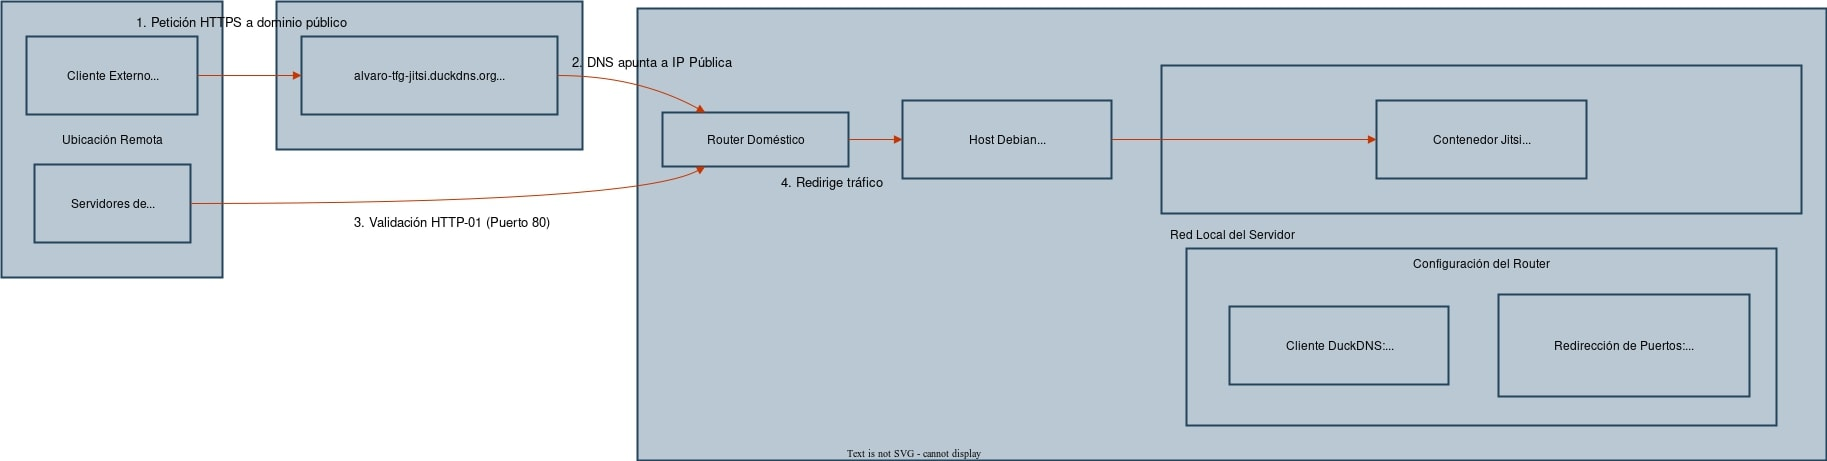
\includegraphics[width=0.9\textwidth]{img/ArquitecturadeRedparaelDesplieguedeJitsi.jpg}
    \caption{Arquitectura de red implementada para permitir el acceso externo seguro vía HTTPS y la validación de certificados de Let's Encrypt.}
    \label{fig:arquitectura_red_letsencrypt}
\end{figure}

\subsection{Certificados Digitales y Autoridades de Certificación}
Para que HTTPS funcione, el servidor debe presentar un \textbf{certificado digital SSL/TLS} que valide su identidad. Existen dos tipos principales:
\begin{itemize}
    \item \textbf{Certificados Autofirmados:} Son generados por el propio administrador del servidor. No son emitidos por una entidad de confianza, por lo que los navegadores web los rechazan por defecto, mostrando advertencias de seguridad al usuario.
    \item \textbf{Certificados de una CA:} Son emitidos por una \textbf{Autoridad de Certificación (CA)}, una entidad externa en la que confían los navegadores (como Let's Encrypt). Cuando un navegador recibe un certificado emitido por una CA de confianza, establece la conexión segura sin advertencias. Por motivos de seguridad, los navegadores modernos exigen una conexión HTTPS con un certificado válido para permitir el acceso a funcionalidades sensibles como la cámara o el micrófono.
\end{itemize}

\section{Componentes Conceptuales de un Pipeline de Datos}
\label{sec:conceptos_pipeline}
Toda arquitectura de procesamiento de datos, como la que se aborda en este proyecto, puede descomponerse en una serie de componentes lógicos, cada uno con una responsabilidad bien definida. La comprensión de estos roles es fundamental para diseñar un sistema robusto y escalable.
\begin{figure}[H]
    \centering
    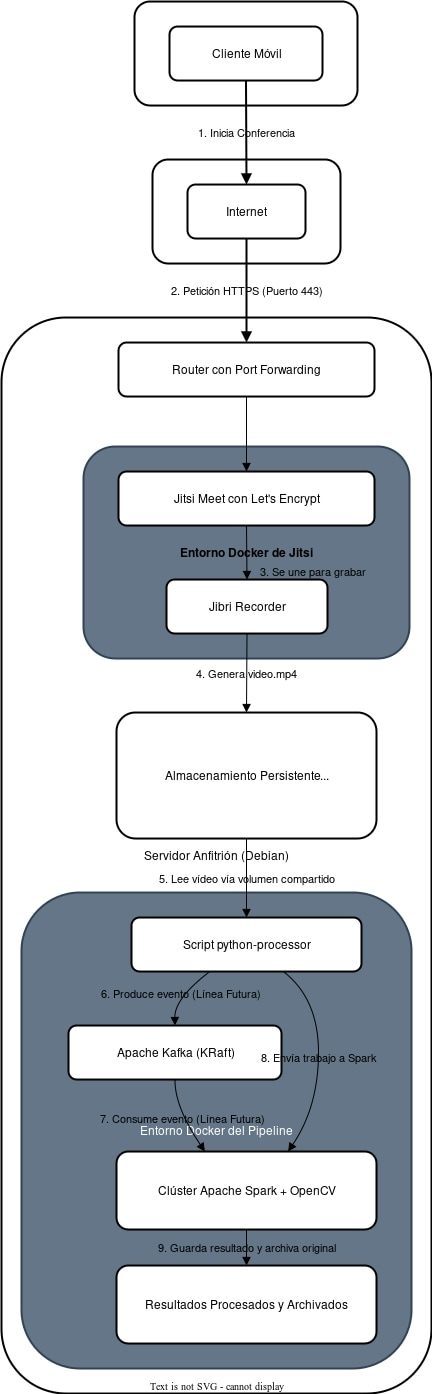
\includegraphics[height=0.9\textheight]{img/arquitectura-general.jpg}
    \caption{Visión general de la arquitectura del sistema, mostrando la interacción entre el subsistema de captura (Jitsi) y el pipeline de procesamiento (Kafka/Spark).}
    \label{fig:arquitectura_completa}
\end{figure}

\subsection{El Productor de Eventos (\textit{Producer})}
El \textbf{Productor} es cualquier entidad del sistema cuya función principal es originar o capturar datos y enviarlos a un sistema de mensajería. Este componente actúa como la fuente de información del pipeline. En el contexto de un sistema de análisis de vídeo, el rol del productor sería desempeñado por el sistema de captura, encargado de digitalizar la sesión y publicarla como un evento o una serie de eventos en el flujo de datos.

\subsection{El Intermediario de Mensajería (\textit{Broker})}
El \textbf{Broker} es el servidor o conjunto de servidores que forman el núcleo del sistema de mensajería. Su responsabilidad es recibir los eventos de los productores, almacenarlos de forma duradera y fiable, y ponerlos a disposición de los consumidores. En arquitecturas distribuidas, se despliega un clúster de brokers para garantizar la alta disponibilidad y la tolerancia a fallos. Este componente es esencial para desacoplar a los productores de los consumidores, permitiendo que operen a ritmos diferentes y de forma independiente.

\subsection{El Consumidor y Procesador de Datos (\textit{Consumer}/\textit{Processor})}
El \textbf{Consumidor} es la aplicación que se suscribe al sistema de mensajería para recibir y leer los eventos que le interesan. Una vez que un consumidor recibe un evento, se lo entrega a una lógica de \textbf{Procesamiento}, que es donde reside la inteligencia de la aplicación. Esta lógica es la que se encarga de transformar, analizar o actuar sobre los datos recibidos. En un sistema de procesamiento de vídeo, el consumidor se encargaría de recibir los datos del vídeo, y el procesador aplicaría los algoritmos de visión artificial sobre ellos.

\subsection{El Modelo de Computación Maestro-Trabajador (\textit{Master-Worker})}
Para procesar grandes volúmenes de datos de manera eficiente, los \textit{frameworks} de computación distribuida suelen emplear el patrón arquitectónico \textbf{Maestro-Trabajador} (conocido también como \textit{Driver-Executor}).
\begin{itemize}
    \item El nodo \textbf{Maestro} (\textit{Master} o \textit{Driver}) es el cerebro de la operación. Recibe el trabajo a realizar, lo divide en un conjunto de tareas más pequeñas e independientes, y las distribuye entre los nodos trabajadores. También se encarga de coordinar la ejecución y agregar los resultados finales.
    \item Los nodos \textbf{Trabajadores} (\textit{Workers} o \textit{Executors}) son los que realizan el trabajo pesado. Cada trabajador recibe una o más tareas del maestro, las ejecuta en paralelo con otros trabajadores sobre una porción de los datos, y devuelve el resultado al maestro.
\end{itemize}
\capitulo{4}{Técnicas y herramientas}

Esta parte de la memoria tiene como objetivo presentar las técnicas metodológicas y las herramientas de desarrollo que se han utilizado para llevar a cabo el proyecto. Si se han estudiado diferentes alternativas de metodologías, herramientas, bibliotecas se puede hacer un resumen de los aspectos más destacados de cada alternativa, incluyendo comparativas entre las distintas opciones y una justificación de las elecciones realizadas. 
No se pretende que este apartado se convierta en un capítulo de un libro dedicado a cada una de las alternativas, sino comentar los aspectos más destacados de cada opción, con un repaso somero a los fundamentos esenciales y referencias bibliográficas para que el lector pueda ampliar su conocimiento sobre el tema.



\capitulo{5}{Aspectos relevantes del desarrollo del proyecto}

Este apartado pretende recoger los aspectos más interesantes del desarrollo del proyecto, comentados por los autores del mismo.
Debe incluir desde la exposición del ciclo de vida utilizado, hasta los detalles de mayor relevancia de las fases de análisis, diseño e implementación.
Se busca que no sea una mera operación de copiar y pegar diagramas y extractos del código fuente, sino que realmente se justifiquen los caminos de solución que se han tomado, especialmente aquellos que no sean triviales.
Puede ser el lugar más adecuado para documentar los aspectos más interesantes del diseño y de la implementación, con un mayor hincapié en aspectos tales como el tipo de arquitectura elegido, los índices de las tablas de la base de datos, normalización y desnormalización, distribución en ficheros3, reglas de negocio dentro de las bases de datos (EDVHV GH GDWRV DFWLYDV), aspectos de desarrollo relacionados con el WWW...
Este apartado, debe convertirse en el resumen de la experiencia práctica del proyecto, y por sí mismo justifica que la memoria se convierta en un documento útil, fuente de referencia para los autores, los tutores y futuros alumnos.

\capitulo{6}{Trabajos relacionados}

Este apartado sería parecido a un estado del arte de una tesis o tesina. En un trabajo final grado no parece obligada su presencia, aunque se puede dejar a juicio del tutor el incluir un pequeño resumen comentado de los trabajos y proyectos ya realizados en el campo del proyecto en curso. 

\chapter{Conclusiones y Líneas de trabajo futuras}
\label{chap:conclusiones}

Para finalizar esta memoria, en este capítulo se presentan, por una parte, las conclusiones principales que he extraído del desarrollo del proyecto y, por otra, las posibles líneas de trabajo futuras que se abren a partir de la infraestructura implementada.

\section{Conclusiones}

La realización de este TFG me ha permitido obtener una serie de conclusiones tanto a nivel técnico como a nivel de gestión y desarrollo de un proyecto de ingeniería de software.

Como primera conclusión, y una de las más importantes, he podido constatar que la \textbf{elección del entorno de desarrollo es crítica} en proyectos que involucran múltiples servicios de red y sistemas de ficheros, como es este caso. El intento inicial de despliegue sobre Windows con WSL2, aunque teóricamente viable, demostró ser una fuente de problemas de compatibilidad (especialmente de permisos y redes) muy difíciles de diagnosticar y resolver. El pivote estratégico a un entorno Linux nativo (Debian 12) fue una decisión fundamental que no solo solucionó los problemas, sino que validó la importancia de trabajar sobre un sistema operativo estándar en entornos de servidor para garantizar la estabilidad y la reproducibilidad.

En segundo lugar, he logrado el objetivo principal de diseñar e implementar una \textbf{arquitectura de datos robusta y escalable}, sentando las bases para un sistema de telerehabilitación mucho más potente que el del proyecto original. La integración de Jitsi, Docker, Kafka y Spark conforma un pipeline de datos modular y desacoplado, que es el estándar de facto en la industria para este tipo de aplicaciones. Aunque la implementación final se ha centrado en un flujo offline, la arquitectura está preparada para evolucionar hacia el procesamiento en tiempo real.

Finalmente, una gran parte del trabajo de ingeniería de este TFG no ha sido la programación de algoritmos complejos, sino la \textbf{integración, configuración y depuración} de múltiples tecnologías de código abierto. Enfrentarme a logs de errores, diagnosticar problemas de red con herramientas como \texttt{openssl}, y comprender las complejas interacciones entre los distintos contenedores ha sido un aprendizaje práctico inmenso y una parte tan valiosa como el propio desarrollo de código.

\section{Líneas de trabajo futuras}

El sistema implementado en este TFG es una base sólida sobre la que se pueden construir numerosas mejoras y nuevas funcionalidades. A continuación, detallo algunas de las líneas de trabajo futuras más interesantes:

\begin{enumerate}
    \item \textbf{Implementar el Pipeline de Streaming en Tiempo Real:} El siguiente paso natural sería evolucionar del procesamiento por lotes (batch) al procesamiento en tiempo real. Esto implicaría configurar Jibri para que emita un flujo de vídeo usando el protocolo RTMP, e implementar un consumidor en Spark Streaming que procese los fotogramas a medida que llegan a través de Kafka.
    
    \item \textbf{Integración con los Algoritmos de Análisis de Movimiento:} Conectar este pipeline de datos con los algoritmos de análisis de esqueletos y DTW desarrollados en los trabajos previos (TFM-FIS-IA y el TFG de Lucía Núñez Calvo). Esto permitiría crear un sistema completo que capture, procese y evalúe los ejercicios de forma totalmente automatizada.
    
    \item \textbf{Escalabilidad y Orquestación Avanzada:} Aunque Docker Compose es ideal para el desarrollo, para un entorno de producción se podría migrar la arquitectura a un orquestador de contenedores más avanzado como \textbf{Kubernetes}. Esto permitiría un escalado automático de los componentes (por ejemplo, añadir más workers de Spark o más instancias de Jibri si hay muchas sesiones concurrentes).
    
    \item \textbf{Monitorización del Sistema:} Desplegar una pila de monitorización (por ejemplo, con \textit{Prometheus} y \textit{Grafana}) para obtener métricas en tiempo real del estado de los brokers de Kafka, los trabajos de Spark y el resto de los servicios, asegurando la salud y el rendimiento del sistema.
\end{enumerate}



\bibliographystyle{plain}
\bibliography{bibliografia}

\end{document}
